\documentclass{standalone}
\usepackage{tikz}
\usetikzlibrary{shapes.geometric, arrows}

\tikzstyle{startstop} = [rectangle, rounded corners, 
minimum width=3cm, 
minimum height=1cm,
text centered, 
draw=black, 
fill=red!30]

\tikzstyle{io} = [trapezium, 
trapezium stretches=true, % A later addition
trapezium left angle=70, 
trapezium right angle=110, 
minimum width=3cm, 
minimum height=1cm, text centered, 
draw=black, fill=blue!30]

\tikzstyle{process} = [rectangle, 
minimum width=3cm, 
minimum height=1cm, 
text centered, 
text width=3cm, 
draw=black, 
fill=orange!30]

\tikzstyle{hidden} = [rectangle, 
minimum width=3cm, 
minimum height=1cm, 
text centered, 
text width=3cm, 
draw=black, 
fill=gray!30]

\tikzstyle{decision} = [diamond, 
minimum width=3cm, 
minimum height=1cm, 
text centered, 
draw=black, 
fill=green!30]

\tikzstyle{arrow} = [thick,->,>=stealth]

\begin{document}

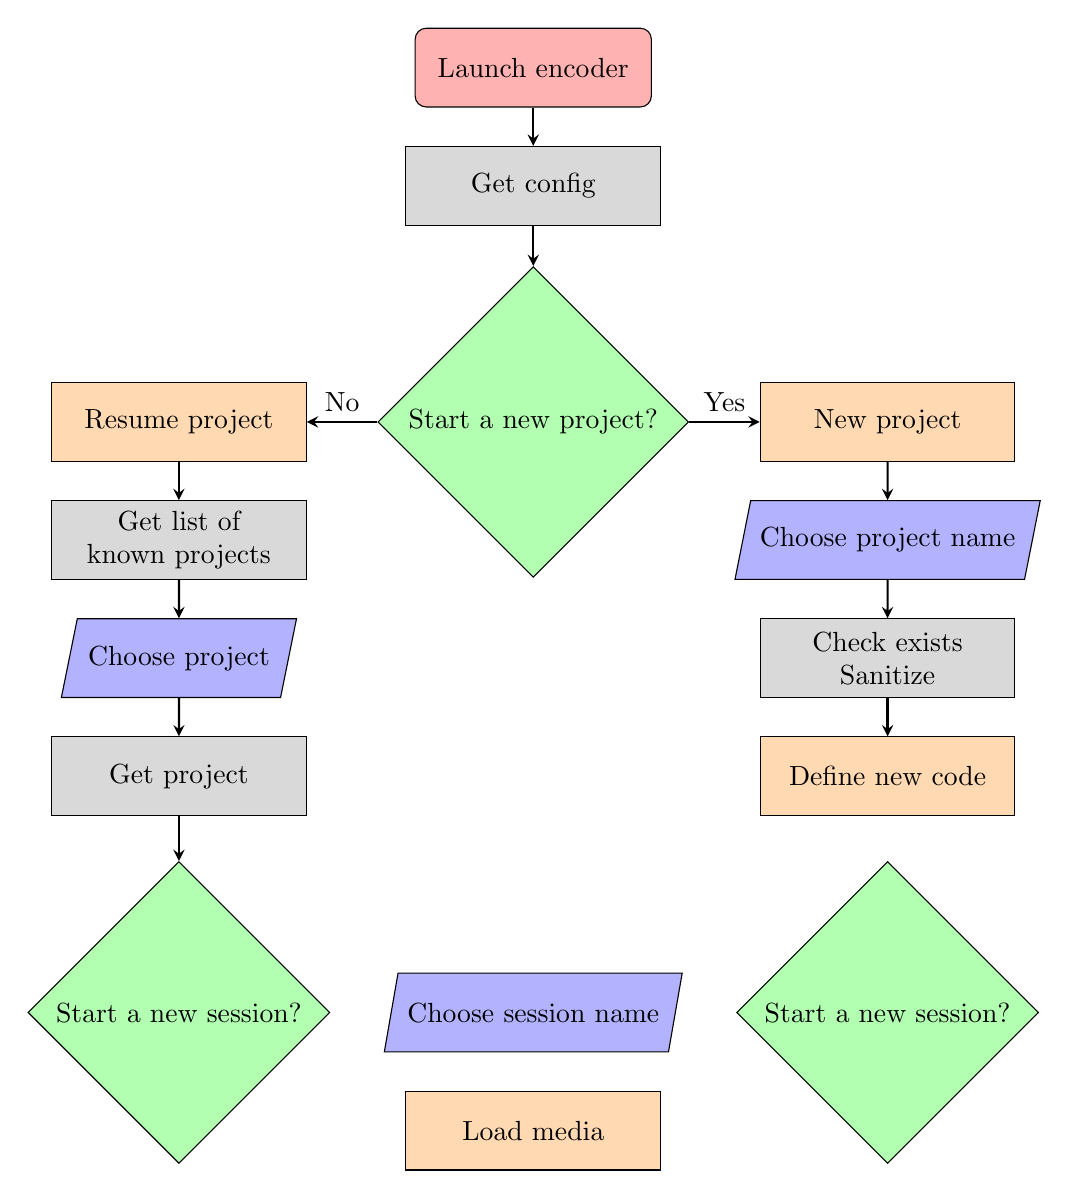
\begin{tikzpicture}[node distance=1.5cm]

\node (launch) [startstop] {Launch encoder};
\node (config) [hidden, below of=launch] {Get config};

\node (dec_project) [decision, below of=config, yshift=-1.5cm] {Start a new project?};

%\node (in1) [io, below of=start] {Input};
\node (new_project) [process, right of=dec_project, xshift=3cm] 
                    {New project};
\node (choose_name) [io, below of=new_project] {Choose project name};
\node (check_name) [hidden, below of=choose_name] 
                   {Check exists\par Sanitize};

\node (new_code) [process, below of=check_name, yshift=0cm] {Define new code};
\node (dec_session_np) [decision, below of=new_code, yshift=-1.5cm] 
                       {Start a new session?};

\node (resume_project) [process, left of=dec_project, xshift=-3cm] 
                       {Resume project};
\node (get_projects) [hidden, below of=resume_project]
                     {Get list of known projects};
\node (choose_project) [io, below of=get_projects] {Choose project};
\node (get_project) [hidden, below of=choose_project] {Get project};

\node (dec_session_rp) [decision, below of=get_project, yshift=-1.5cm] {Start a new
session?};

\node (choose_session) [io, right of=dec_session_rp, xshift=3cm]{Choose session name};

\node (load_media) [process, below of=choose_session, yshift=0cm] {Load media};

%\node (pro2a) [process, below of=dec1, yshift=-0.5cm] {Process 2a
%text text text text
%text text text 
%text text text};
%
%%\node (pro2b) [process, right of=dec1, xshift=2cm] {Process 2b};
%\node (out1) [io, below of=pro2a] {Output};
%\node (stop) [startstop, below of=out1] {Stop};

\draw [arrow] (launch) -- (config);
\draw [arrow] (config) -- (dec_project);
%\draw [arrow] (in1) -- (pro1);
\draw [arrow] (dec_project) -- node[anchor=south] {Yes} (new_project);
\draw [arrow] (dec_project) -- node[anchor=south] {No} (resume_project);
\draw [arrow] (new_project) -- (choose_name);
\draw [arrow] (choose_name) -- (check_name);
\draw [arrow] (check_name) -- (new_code);
%\draw [arrow] (new_code) -- (load_media);
\draw [arrow] (resume_project) -- (get_projects);
\draw [arrow] (get_projects) -- (choose_project);
\draw [arrow] (choose_project) -- (get_project);
\draw [arrow] (get_project) -- (dec_session_rp);

%\draw [arrow] (pro2b) |- (pro1);
%\draw [arrow] (pro2a) -- (out1);
%\draw [arrow] (out1) -- (stop);

\end{tikzpicture}
\end{document}
